\section{Auswertung}
\label{sec:Auswertung}
\subsection{Bestimmung des Schubmoduls G}
\begin{equation}
	\theta_{\mathrm{Kugel}}=(1.3197\pm 0.0006) \cdot 10^{-4} \,\si{\kilo\gram \square\metre}
\end{equation}
\begin{equation}
	G= (8.987\pm 0.004) \cdot 10^{10}  \,\si{\newton \per \square\metre}
\end{equation}
\begin{equation}
	Q= (1.056\pm 0.011) \cdot 10^{11}  \,\si{\newton \per \square\metre}
\end{equation}

\begin{equation}
	\mu= 0.1684\pm 0.0028
\end{equation}
%\begin{figure}
%  \centering
%  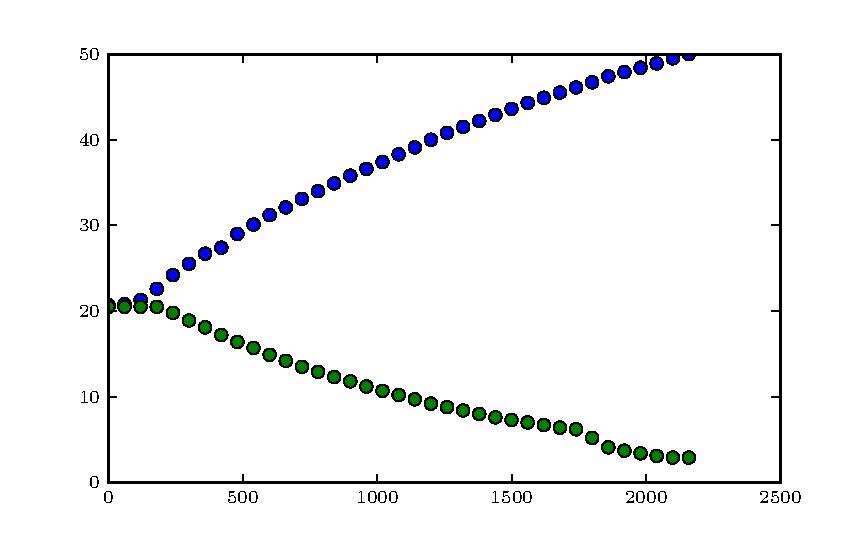
\includegraphics{plot.pdf}
%  \caption{Plot.}
%  \label{fig:plot}
%\end{figure}
E= (2.100+/-0.005)e+11
\subsection{Bestimmung des magnetischen Moments $m$ des Helmholtzspulenpaars}
Das B-Feld eines Helmholtzspulenpaars ergibt sich mit
\begin{equation}
	B_{\mathrm{H}}=
\end{equation}



a = m = 0.0338563481372 +- 0.000438666200483
b = D =  7.434181548e-06 +- 1.22371249137e-06
